%%%%%%%%%%%%%%%%%%%%%%%%%%%%%%%%%%%%%%%%%%%%%%%%%%%%%%%%%%%%%%%%%%%%%%%%%%%%%%%%%%%%%%%%%%%%%%%%%
%
% Document:     Data Management  product tree
%
%%%%%%%%%%%%%%%%%%%%%%%%%%%%%%%%%%%%%%%%%%%%%%%%%%%%%%%%%%%%%%%%%%%%%%%%%%%%%%
\documentclass{article}
\usepackage{times,layouts}
\usepackage{tikz,hyperref,amsmath}
\usetikzlibrary{positioning,arrows,shapes,decorations.shapes,shapes.arrows}
\usetikzlibrary{backgrounds,calc}
\usepackage[paperwidth=1702.0pt,paperheight=2236pt,
left=-2mm,top=3mm,bottom=0mm,right=0mm,
noheadfoot,marginparwidth=0pt,includemp=false,
textwidth=30cm,textheight=50mm]{geometry}
\newcommand\showpage{%
\setlayoutscale{0.5}\setlabelfont{\tiny}\printheadingsfalse\printparametersfalse
\currentpage\pagedesign}
\hypersetup{pdftitle={Data Management products }, pdfsubject={Diagram illustrating the
                products in LSST Data Management }, pdfauthor={Extracted from MagicDraw}}
\tikzstyle{tbox}=[rectangle,text centered, text width=30mm]
\tikzstyle{wbbox}=[rectangle, rounded corners=3pt, draw=black, top color=blue!50!white,
                    bottom color=white, very thick, minimum height=40pt, inner sep=2pt,
                    text centered, text width=30mm]
\tikzstyle{pbox}=[rectangle, rounded corners=3pt, draw=black, top
 color=yellow!50!white, bottom color=white, very thick,
 minimum height=36pt, inner sep=3pt, text centered, text width=35mm]
\tikzstyle{pline}=[-, thick]
\begin{document}
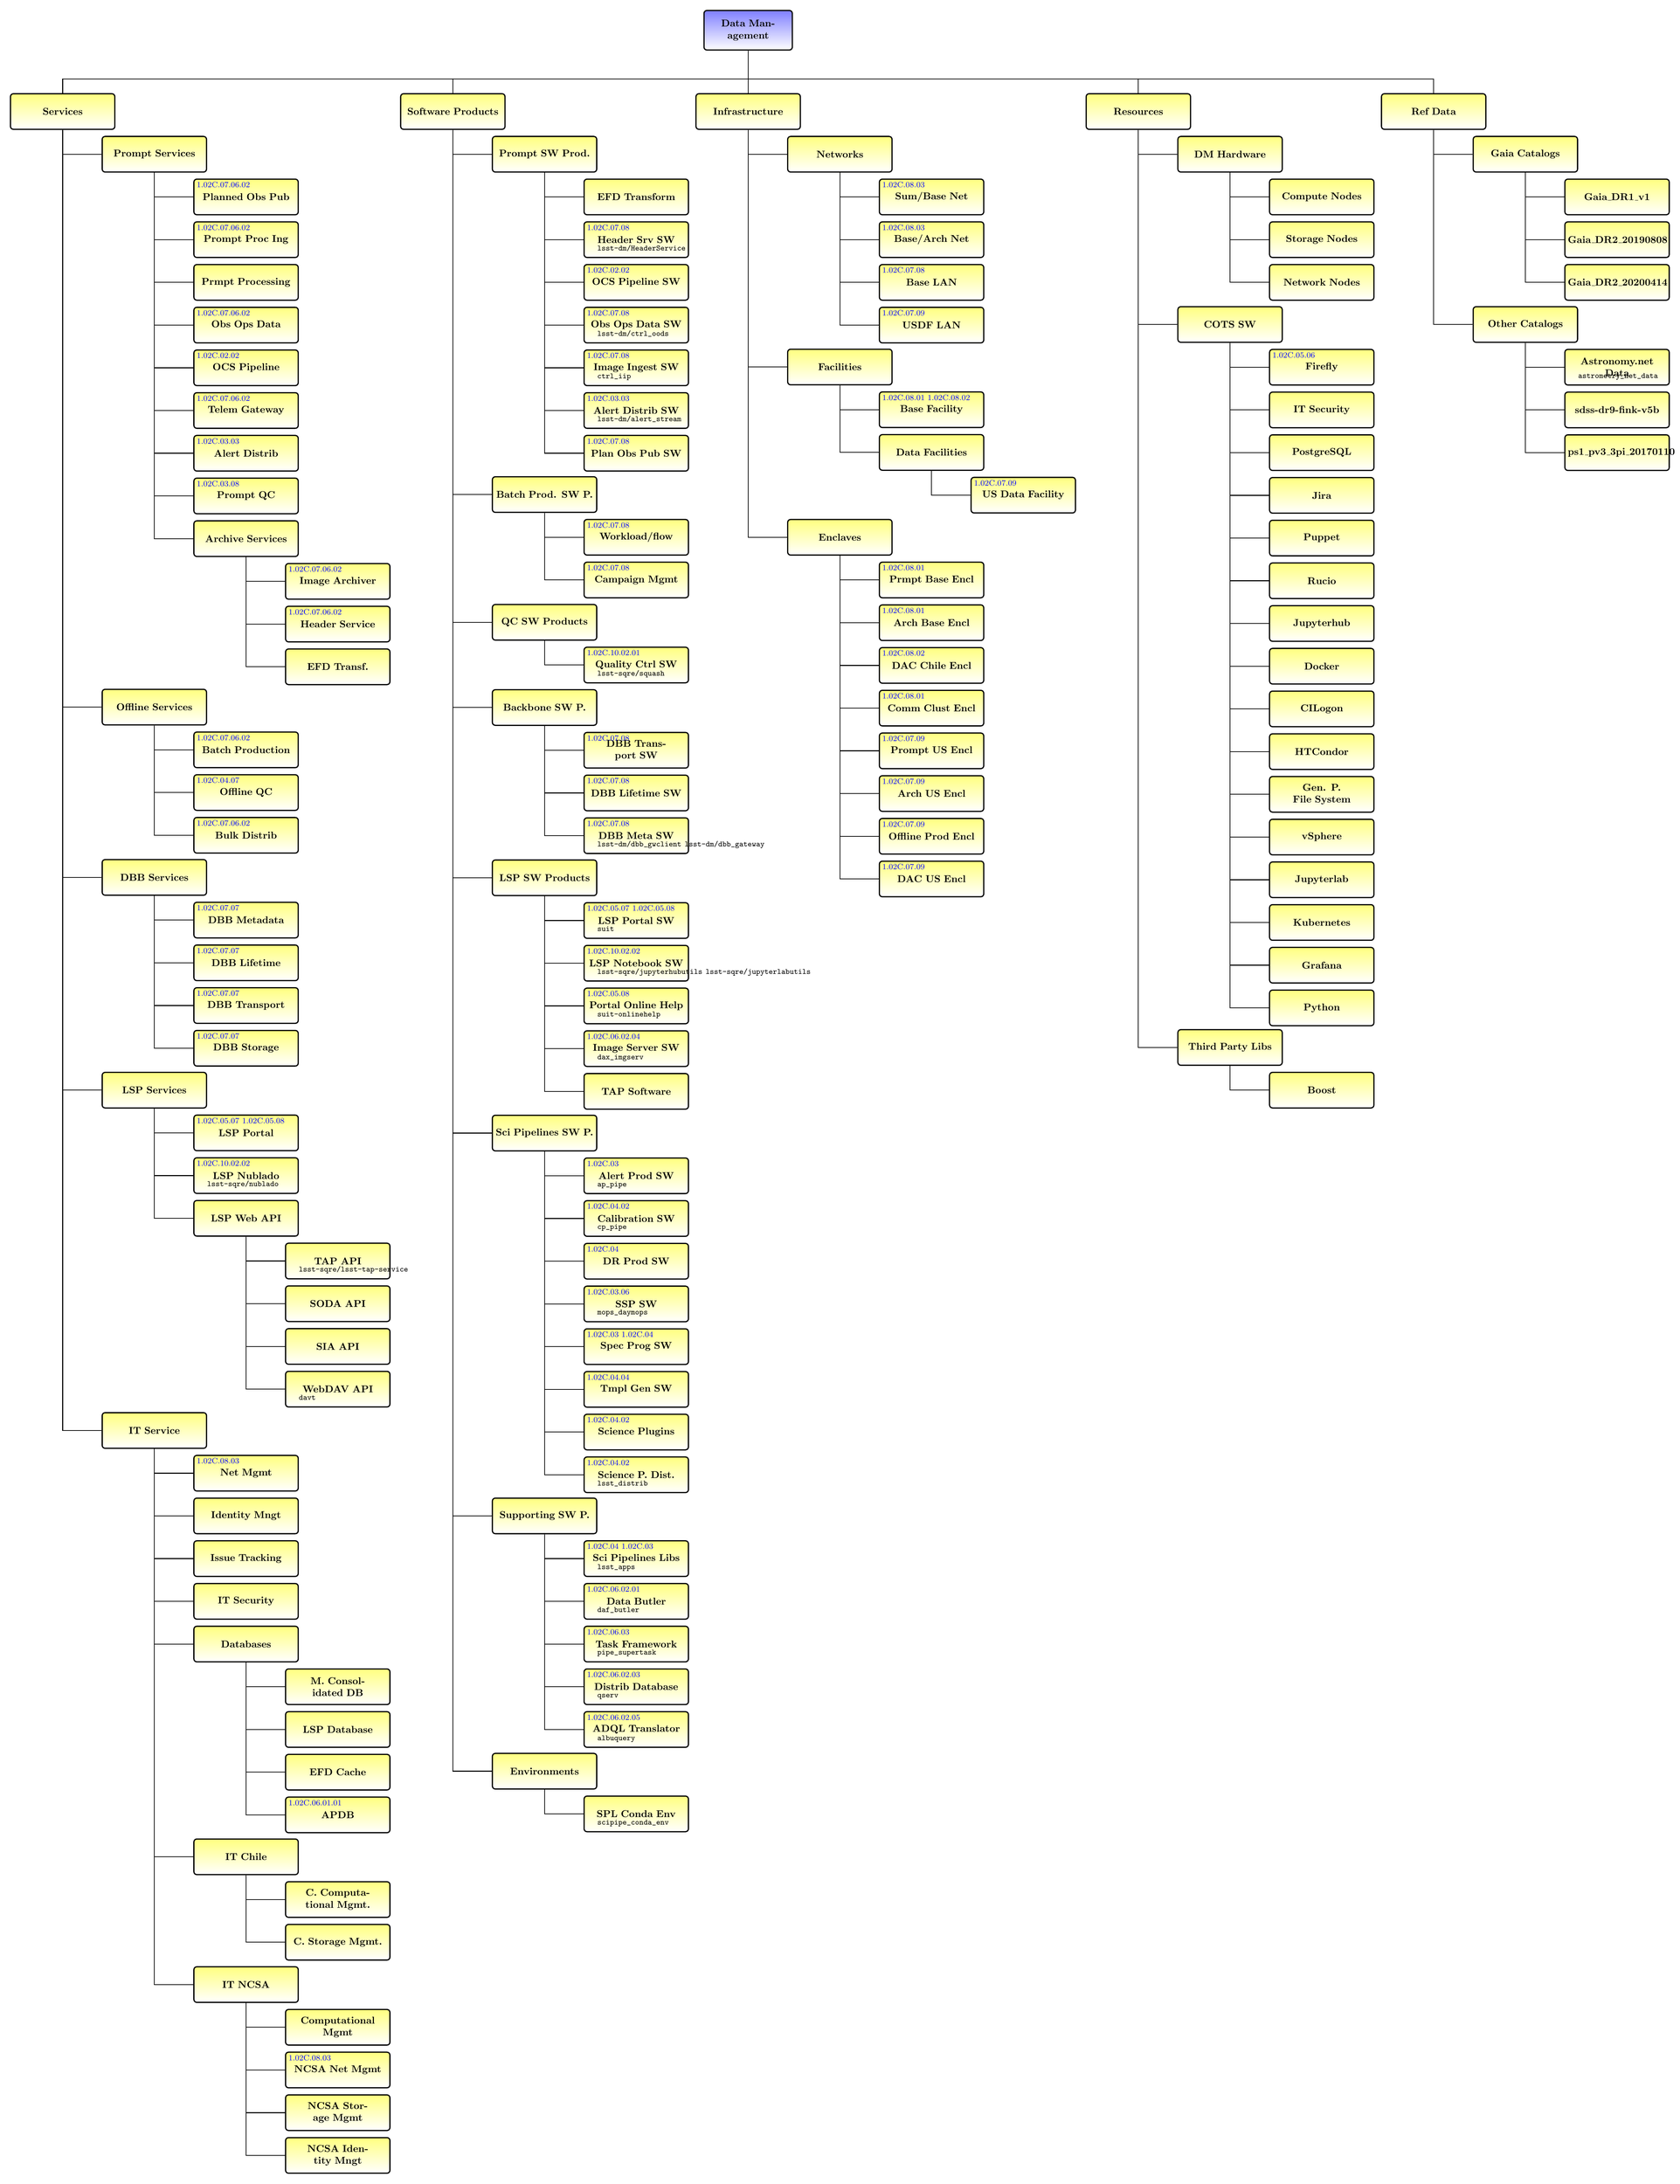
\begin{tikzpicture}[node distance=0mm]


\node (DMSRV) [pbox, 
] {\textbf{Services
} };\node [below right] at (DMSRV.north west) {\footnotesize \color{blue}} ;

\node (PRSRV) [pbox,below right=6pt and -14pt of DMSRV] {\textbf{Prompt Services
} };\node [below right] at (PRSRV.north west) {\footnotesize \color{blue}} ;

 \draw[pline] (DMSRV.south) -| ++(0,0) |- (PRSRV.west); 
\node (POPSRV) [pbox,below right=6pt and -14pt of PRSRV] {\textbf{Planned Obs Pub
} };\node [below right] at (POPSRV.north west) {\footnotesize \color{blue}1.02C.07.06.02} ;

 \draw[pline] (PRSRV.south) -| ++(0,0) |- (POPSRV.west); 
\node (PRPINGSRV) [pbox,below=6pt of POPSRV] {\textbf{Prompt Proc Ing
} };\node [below right] at (PRPINGSRV.north west) {\footnotesize \color{blue}1.02C.07.06.02} ;

 \draw[pline] (PRSRV.south) -| ++(0,0) |- (PRPINGSRV.west); 
\node (PRPRSRV) [pbox,below=6pt of PRPINGSRV] {\textbf{Prmpt Processing
} };\node [below right] at (PRPRSRV.north west) {\footnotesize \color{blue}} ;

 \draw[pline] (PRSRV.south) -| ++(0,0) |- (PRPRSRV.west); 
\node (OODSSRV) [pbox,below=6pt of PRPRSRV] {\textbf{Obs Ops Data
} };\node [below right] at (OODSSRV.north west) {\footnotesize \color{blue}1.02C.07.06.02} ;

 \draw[pline] (PRSRV.south) -| ++(0,0) |- (OODSSRV.west); 
\node (OCPSRV) [pbox,below=6pt of OODSSRV] {\textbf{OCS Pipeline
} };\node [below right] at (OCPSRV.north west) {\footnotesize \color{blue}1.02C.02.02} ;

 \draw[pline] (PRSRV.south) -| ++(0,0) |- (OCPSRV.west); 
\node (TMGSRV) [pbox,below=6pt of OCPSRV] {\textbf{Telem Gateway
} };\node [below right] at (TMGSRV.north west) {\footnotesize \color{blue}1.02C.07.06.02} ;

 \draw[pline] (PRSRV.south) -| ++(0,0) |- (TMGSRV.west); 
\node (ALRTDSTSRV) [pbox,below=6pt of TMGSRV] {\textbf{Alert Distrib
} };\node [below right] at (ALRTDSTSRV.north west) {\footnotesize \color{blue}1.02C.03.03} ;

 \draw[pline] (PRSRV.south) -| ++(0,0) |- (ALRTDSTSRV.west); 
\node (PRQCSRV) [pbox,below=6pt of ALRTDSTSRV] {\textbf{Prompt QC
} };\node [below right] at (PRQCSRV.north west) {\footnotesize \color{blue}1.02C.03.08} ;

 \draw[pline] (PRSRV.south) -| ++(0,0) |- (PRQCSRV.west); 
\node (ARCSRVS) [pbox,below=6pt of PRQCSRV] {\textbf{Archive Services
} };\node [below right] at (ARCSRVS.north west) {\footnotesize \color{blue}} ;

 \draw[pline] (PRSRV.south) -| ++(0,0) |- (ARCSRVS.west); 
\node (IMAS) [pbox,below right=6pt and -14pt of ARCSRVS] {\textbf{Image Archiver
} };\node [below right] at (IMAS.north west) {\footnotesize \color{blue}1.02C.07.06.02} ;

 \draw[pline] (ARCSRVS.south) -| ++(0,0) |- (IMAS.west); 
\node (HEADS) [pbox,below=6pt of IMAS] {\textbf{Header Service
} };\node [below right] at (HEADS.north west) {\footnotesize \color{blue}1.02C.07.06.02} ;

 \draw[pline] (ARCSRVS.south) -| ++(0,0) |- (HEADS.west); 
\node (EFDTS) [pbox,below=6pt of HEADS] {\textbf{EFD Transf.
} };\node [below right] at (EFDTS.north west) {\footnotesize \color{blue}} ;

 \draw[pline] (ARCSRVS.south) -| ++(0,0) |- (EFDTS.west); 
\node (OFFLSRV) [pbox,below=522pt of PRSRV] {\textbf{Offline Services
} };\node [below right] at (OFFLSRV.north west) {\footnotesize \color{blue}} ;

 \draw[pline] (DMSRV.south) -| ++(0,0) |- (OFFLSRV.west); 
\node (PRODSRV) [pbox,below right=6pt and -14pt of OFFLSRV] {\textbf{Batch Production
} };\node [below right] at (PRODSRV.north west) {\footnotesize \color{blue}1.02C.07.06.02} ;

 \draw[pline] (OFFLSRV.south) -| ++(0,0) |- (PRODSRV.west); 
\node (OFFLQCSRV) [pbox,below=6pt of PRODSRV] {\textbf{Offline QC
} };\node [below right] at (OFFLQCSRV.north west) {\footnotesize \color{blue}1.02C.04.07} ;

 \draw[pline] (OFFLSRV.south) -| ++(0,0) |- (OFFLQCSRV.west); 
\node (BULKDSRV) [pbox,below=6pt of OFFLQCSRV] {\textbf{Bulk Distrib
} };\node [below right] at (BULKDSRV.north west) {\footnotesize \color{blue}1.02C.07.06.02} ;

 \draw[pline] (OFFLSRV.south) -| ++(0,0) |- (BULKDSRV.west); 
\node (DBBSRV) [pbox,below=135pt of OFFLSRV] {\textbf{DBB Services
} };\node [below right] at (DBBSRV.north west) {\footnotesize \color{blue}} ;

 \draw[pline] (DMSRV.south) -| ++(0,0) |- (DBBSRV.west); 
\node (DBBMDSRV) [pbox,below right=6pt and -14pt of DBBSRV] {\textbf{DBB Metadata
} };\node [below right] at (DBBMDSRV.north west) {\footnotesize \color{blue}1.02C.07.07} ;

 \draw[pline] (DBBSRV.south) -| ++(0,0) |- (DBBMDSRV.west); 
\node (DBBLIFESRV) [pbox,below=6pt of DBBMDSRV] {\textbf{DBB Lifetime
} };\node [below right] at (DBBLIFESRV.north west) {\footnotesize \color{blue}1.02C.07.07} ;

 \draw[pline] (DBBSRV.south) -| ++(0,0) |- (DBBLIFESRV.west); 
\node (DBBTRSRV) [pbox,below=6pt of DBBLIFESRV] {\textbf{DBB Transport
} };\node [below right] at (DBBTRSRV.north west) {\footnotesize \color{blue}1.02C.07.07} ;

 \draw[pline] (DBBSRV.south) -| ++(0,0) |- (DBBTRSRV.west); 
\node (DBBSTRSRV) [pbox,below=6pt of DBBTRSRV] {\textbf{DBB Storage
} };\node [below right] at (DBBSTRSRV.north west) {\footnotesize \color{blue}1.02C.07.07} ;

 \draw[pline] (DBBSRV.south) -| ++(0,0) |- (DBBSTRSRV.west); 
\node (LSPSRV) [pbox,below=178pt of DBBSRV] {\textbf{LSP Services
} };\node [below right] at (LSPSRV.north west) {\footnotesize \color{blue}} ;

 \draw[pline] (DMSRV.south) -| ++(0,0) |- (LSPSRV.west); 
\node (PRTLSRV) [pbox,below right=6pt and -14pt of LSPSRV] {\textbf{LSP Portal
} };\node [below right] at (PRTLSRV.north west) {\footnotesize \color{blue}1.02C.05.07 1.02C.05.08} ;

 \draw[pline] (LSPSRV.south) -| ++(0,0) |- (PRTLSRV.west); 
\node (NBLSRV) [pbox,below=6pt of PRTLSRV] {\textbf{LSP Nublado
} };\node [below right] at (NBLSRV.north west) {\footnotesize \color{blue}1.02C.10.02.02} ;
\node (NBLSRVpkg) [tbox,below=3mm of NBLSRV.north] {{\footnotesize \color{black} \begin{verbatim} lsst-sqre/nublado \end{verbatim} }  };

 \draw[pline] (LSPSRV.south) -| ++(0,0) |- (NBLSRV.west); 
\node (LSPWAPI) [pbox,below=6pt of NBLSRV] {\textbf{LSP Web API
} };\node [below right] at (LSPWAPI.north west) {\footnotesize \color{blue}} ;

 \draw[pline] (LSPSRV.south) -| ++(0,0) |- (LSPWAPI.west); 
\node (TAPSRV) [pbox,below right=6pt and -14pt of LSPWAPI] {\textbf{TAP API
} };\node [below right] at (TAPSRV.north west) {\footnotesize \color{blue}} ;
\node (TAPSRVpkg) [tbox,below=3mm of TAPSRV.north] {{\footnotesize \color{black} \begin{verbatim} lsst-sqre/lsst-tap-service \end{verbatim} }  };

 \draw[pline] (LSPWAPI.south) -| ++(0,0) |- (TAPSRV.west); 
\node (SODASRV) [pbox,below=6pt of TAPSRV] {\textbf{SODA API
} };\node [below right] at (SODASRV.north west) {\footnotesize \color{blue}} ;

 \draw[pline] (LSPWAPI.south) -| ++(0,0) |- (SODASRV.west); 
\node (SIASRV) [pbox,below=6pt of SODASRV] {\textbf{SIA API
} };\node [below right] at (SIASRV.north west) {\footnotesize \color{blue}} ;

 \draw[pline] (LSPWAPI.south) -| ++(0,0) |- (SIASRV.west); 
\node (WDAVSRV) [pbox,below=6pt of SIASRV] {\textbf{WebDAV API
} };\node [below right] at (WDAVSRV.north west) {\footnotesize \color{blue}} ;
\node (WDAVSRVpkg) [tbox,below=3mm of WDAVSRV.north] {{\footnotesize \color{black} \begin{verbatim} davt \end{verbatim} }  };

 \draw[pline] (LSPWAPI.south) -| ++(0,0) |- (WDAVSRV.west); 
\node (ITSRV) [pbox,below=307pt of LSPSRV] {\textbf{IT Service
} };\node [below right] at (ITSRV.north west) {\footnotesize \color{blue}} ;

 \draw[pline] (DMSRV.south) -| ++(0,0) |- (ITSRV.west); 
\node (NETMGMT) [pbox,below right=6pt and -14pt of ITSRV] {\textbf{Net Mgmt
} };\node [below right] at (NETMGMT.north west) {\footnotesize \color{blue}1.02C.08.03} ;

 \draw[pline] (ITSRV.south) -| ++(0,0) |- (NETMGMT.west); 
\node (IDNMNG) [pbox,below=6pt of NETMGMT] {\textbf{Identity Mngt
} };\node [below right] at (IDNMNG.north west) {\footnotesize \color{blue}} ;

 \draw[pline] (ITSRV.south) -| ++(0,0) |- (IDNMNG.west); 
\node (ITRCK) [pbox,below=6pt of IDNMNG] {\textbf{Issue Tracking
} };\node [below right] at (ITRCK.north west) {\footnotesize \color{blue}} ;

 \draw[pline] (ITSRV.south) -| ++(0,0) |- (ITRCK.west); 
\node (ITSEC) [pbox,below=6pt of ITRCK] {\textbf{IT Security
} };\node [below right] at (ITSEC.north west) {\footnotesize \color{blue}} ;

 \draw[pline] (ITSRV.south) -| ++(0,0) |- (ITSEC.west); 
\node (MNGDB) [pbox,below=6pt of ITSEC] {\textbf{Databases
} };\node [below right] at (MNGDB.north west) {\footnotesize \color{blue}} ;

 \draw[pline] (ITSRV.south) -| ++(0,0) |- (MNGDB.west); 
\node (MCDB) [pbox,below right=6pt and -14pt of MNGDB] {\textbf{M. Consolidated DB
} };\node [below right] at (MCDB.north west) {\footnotesize \color{blue}} ;

 \draw[pline] (MNGDB.south) -| ++(0,0) |- (MCDB.west); 
\node (LSPDB) [pbox,below=6pt of MCDB] {\textbf{LSP Database
} };\node [below right] at (LSPDB.north west) {\footnotesize \color{blue}} ;

 \draw[pline] (MNGDB.south) -| ++(0,0) |- (LSPDB.west); 
\node (EFDB) [pbox,below=6pt of LSPDB] {\textbf{EFD Cache
} };\node [below right] at (EFDB.north west) {\footnotesize \color{blue}} ;

 \draw[pline] (MNGDB.south) -| ++(0,0) |- (EFDB.west); 
\node (APDB) [pbox,below=6pt of EFDB] {\textbf{APDB
} };\node [below right] at (APDB.north west) {\footnotesize \color{blue}1.02C.06.01.01} ;

 \draw[pline] (MNGDB.south) -| ++(0,0) |- (APDB.west); 
\node (ITCH) [pbox,below=178pt of MNGDB] {\textbf{IT Chile
} };\node [below right] at (ITCH.north west) {\footnotesize \color{blue}} ;

 \draw[pline] (ITSRV.south) -| ++(0,0) |- (ITCH.west); 
\node (CHCNM) [pbox,below right=6pt and -14pt of ITCH] {\textbf{C. Computational Mgmt.
} };\node [below right] at (CHCNM.north west) {\footnotesize \color{blue}} ;

 \draw[pline] (ITCH.south) -| ++(0,0) |- (CHCNM.west); 
\node (CHSTMNG) [pbox,below=6pt of CHCNM] {\textbf{C. Storage Mgmt.
} };\node [below right] at (CHSTMNG.north west) {\footnotesize \color{blue}} ;

 \draw[pline] (ITCH.south) -| ++(0,0) |- (CHSTMNG.west); 
\node (ITNCSA) [pbox,below=92pt of ITCH] {\textbf{IT NCSA
} };\node [below right] at (ITNCSA.north west) {\footnotesize \color{blue}} ;

 \draw[pline] (ITSRV.south) -| ++(0,0) |- (ITNCSA.west); 
\node (NCSACNM) [pbox,below right=6pt and -14pt of ITNCSA] {\textbf{Computational Mgmt
} };\node [below right] at (NCSACNM.north west) {\footnotesize \color{blue}} ;

 \draw[pline] (ITNCSA.south) -| ++(0,0) |- (NCSACNM.west); 
\node (NCSANETMNG) [pbox,below=6pt of NCSACNM] {\textbf{NCSA Net Mgmt
} };\node [below right] at (NCSANETMNG.north west) {\footnotesize \color{blue}1.02C.08.03} ;

 \draw[pline] (ITNCSA.south) -| ++(0,0) |- (NCSANETMNG.west); 
\node (NCSASTMNG) [pbox,below=6pt of NCSANETMNG] {\textbf{NCSA Storage Mgmt
} };\node [below right] at (NCSASTMNG.north west) {\footnotesize \color{blue}} ;

 \draw[pline] (ITNCSA.south) -| ++(0,0) |- (NCSASTMNG.west); 
\node (NCSAIDNMNG) [pbox,below=6pt of NCSASTMNG] {\textbf{NCSA Identity Mngt
} };\node [below right] at (NCSAIDNMNG.north west) {\footnotesize \color{blue}} ;

 \draw[pline] (ITNCSA.south) -| ++(0,0) |- (NCSAIDNMNG.west); 
\node (DMSW) [pbox, 
right=288pt of DMSRV] {\textbf{Software Products
} };\node [below right] at (DMSW.north west) {\footnotesize \color{blue}} ;

\node (PRSW) [pbox,below right=6pt and -14pt of DMSW] {\textbf{Prompt SW Prod.
} };\node [below right] at (PRSW.north west) {\footnotesize \color{blue}} ;

 \draw[pline] (DMSW.south) -| ++(0,0) |- (PRSW.west); 
\node (EFDT) [pbox,below right=6pt and -14pt of PRSW] {\textbf{EFD Transform
} };\node [below right] at (EFDT.north west) {\footnotesize \color{blue}} ;

 \draw[pline] (PRSW.south) -| ++(0,0) |- (EFDT.west); 
\node (HEADER) [pbox,below=6pt of EFDT] {\textbf{Header Srv SW
} };\node [below right] at (HEADER.north west) {\footnotesize \color{blue}1.02C.07.08} ;
\node (HEADERpkg) [tbox,below=3mm of HEADER.north] {{\footnotesize \color{black} \begin{verbatim} lsst-dm/HeaderService \end{verbatim} }  };

 \draw[pline] (PRSW.south) -| ++(0,0) |- (HEADER.west); 
\node (OCPS) [pbox,below=6pt of HEADER] {\textbf{OCS Pipeline SW
} };\node [below right] at (OCPS.north west) {\footnotesize \color{blue}1.02C.02.02} ;

 \draw[pline] (PRSW.south) -| ++(0,0) |- (OCPS.west); 
\node (OODS) [pbox,below=6pt of OCPS] {\textbf{Obs Ops Data SW
} };\node [below right] at (OODS.north west) {\footnotesize \color{blue}1.02C.07.08} ;
\node (OODSpkg) [tbox,below=3mm of OODS.north] {{\footnotesize \color{black} \begin{verbatim} lsst-dm/ctrl_oods \end{verbatim} }  };

 \draw[pline] (PRSW.south) -| ++(0,0) |- (OODS.west); 
\node (IIP) [pbox,below=6pt of OODS] {\textbf{Image Ingest SW
} };\node [below right] at (IIP.north west) {\footnotesize \color{blue}1.02C.07.08} ;
\node (IIPpkg) [tbox,below=3mm of IIP.north] {{\footnotesize \color{black} \begin{verbatim} ctrl_iip \end{verbatim} }  };

 \draw[pline] (PRSW.south) -| ++(0,0) |- (IIP.west); 
\node (ALRTDSTR) [pbox,below=6pt of IIP] {\textbf{Alert Distrib SW
} };\node [below right] at (ALRTDSTR.north west) {\footnotesize \color{blue}1.02C.03.03} ;
\node (ALRTDSTRpkg) [tbox,below=3mm of ALRTDSTR.north] {{\footnotesize \color{black} \begin{verbatim} lsst-dm/alert_stream \end{verbatim} }  };

 \draw[pline] (PRSW.south) -| ++(0,0) |- (ALRTDSTR.west); 
\node (OBSPUB) [pbox,below=6pt of ALRTDSTR] {\textbf{Plan Obs Pub SW
} };\node [below right] at (OBSPUB.north west) {\footnotesize \color{blue}1.02C.07.08} ;

 \draw[pline] (PRSW.south) -| ++(0,0) |- (OBSPUB.west); 
\node (BPSWP) [pbox,below=307pt of PRSW] {\textbf{Batch Prod. SW P.
} };\node [below right] at (BPSWP.north west) {\footnotesize \color{blue}} ;

 \draw[pline] (DMSW.south) -| ++(0,0) |- (BPSWP.west); 
\node (WLWF) [pbox,below right=6pt and -14pt of BPSWP] {\textbf{Workload/flow
} };\node [below right] at (WLWF.north west) {\footnotesize \color{blue}1.02C.07.08} ;

 \draw[pline] (BPSWP.south) -| ++(0,0) |- (WLWF.west); 
\node (CMPGN) [pbox,below=6pt of WLWF] {\textbf{Campaign Mgmt
} };\node [below right] at (CMPGN.north west) {\footnotesize \color{blue}1.02C.07.08} ;

 \draw[pline] (BPSWP.south) -| ++(0,0) |- (CMPGN.west); 
\node (QCSWP) [pbox,below=92pt of BPSWP] {\textbf{QC SW Products
} };\node [below right] at (QCSWP.north west) {\footnotesize \color{blue}} ;

 \draw[pline] (DMSW.south) -| ++(0,0) |- (QCSWP.west); 
\node (QCSW) [pbox,below right=6pt and -14pt of QCSWP] {\textbf{Quality Ctrl SW
} };\node [below right] at (QCSW.north west) {\footnotesize \color{blue}1.02C.10.02.01} ;
\node (QCSWpkg) [tbox,below=3mm of QCSW.north] {{\footnotesize \color{black} \begin{verbatim} lsst-sqre/squash \end{verbatim} }  };

 \draw[pline] (QCSWP.south) -| ++(0,0) |- (QCSW.west); 
\node (BBSWP) [pbox,below=49pt of QCSWP] {\textbf{Backbone SW P.
} };\node [below right] at (BBSWP.north west) {\footnotesize \color{blue}} ;

 \draw[pline] (DMSW.south) -| ++(0,0) |- (BBSWP.west); 
\node (DBBTR) [pbox,below right=6pt and -14pt of BBSWP] {\textbf{DBB Transport SW
} };\node [below right] at (DBBTR.north west) {\footnotesize \color{blue}1.02C.07.08} ;

 \draw[pline] (BBSWP.south) -| ++(0,0) |- (DBBTR.west); 
\node (DBBLIFE) [pbox,below=6pt of DBBTR] {\textbf{DBB Lifetime SW
} };\node [below right] at (DBBLIFE.north west) {\footnotesize \color{blue}1.02C.07.08} ;

 \draw[pline] (BBSWP.south) -| ++(0,0) |- (DBBLIFE.west); 
\node (DBBMD) [pbox,below=6pt of DBBLIFE] {\textbf{DBB Meta SW
} };\node [below right] at (DBBMD.north west) {\footnotesize \color{blue}1.02C.07.08} ;
\node (DBBMDpkg) [tbox,below=3mm of DBBMD.north] {{\footnotesize \color{black} \begin{verbatim} lsst-dm/dbb_gwclient lsst-dm/dbb_gateway \end{verbatim} }  };

 \draw[pline] (BBSWP.south) -| ++(0,0) |- (DBBMD.west); 
\node (LSPSWP) [pbox,below=135pt of BBSWP] {\textbf{LSP SW Products
} };\node [below right] at (LSPSWP.north west) {\footnotesize \color{blue}} ;

 \draw[pline] (DMSW.south) -| ++(0,0) |- (LSPSWP.west); 
\node (PRTLSW) [pbox,below right=6pt and -14pt of LSPSWP] {\textbf{LSP Portal SW
} };\node [below right] at (PRTLSW.north west) {\footnotesize \color{blue}1.02C.05.07 1.02C.05.08} ;
\node (PRTLSWpkg) [tbox,below=3mm of PRTLSW.north] {{\footnotesize \color{black} \begin{verbatim} suit \end{verbatim} }  };

 \draw[pline] (LSPSWP.south) -| ++(0,0) |- (PRTLSW.west); 
\node (NBSW) [pbox,below=6pt of PRTLSW] {\textbf{LSP Notebook SW
} };\node [below right] at (NBSW.north west) {\footnotesize \color{blue}1.02C.10.02.02} ;
\node (NBSWpkg) [tbox,below=3mm of NBSW.north] {{\footnotesize \color{black} \begin{verbatim} lsst-sqre/jupyterhubutils lsst-sqre/jupyterlabutils \end{verbatim} }  };

 \draw[pline] (LSPSWP.south) -| ++(0,0) |- (NBSW.west); 
\node (PRTLOH) [pbox,below=6pt of NBSW] {\textbf{Portal Online Help
} };\node [below right] at (PRTLOH.north west) {\footnotesize \color{blue}1.02C.05.08} ;
\node (PRTLOHpkg) [tbox,below=3mm of PRTLOH.north] {{\footnotesize \color{black} \begin{verbatim} suit-onlinehelp \end{verbatim} }  };

 \draw[pline] (LSPSWP.south) -| ++(0,0) |- (PRTLOH.west); 
\node (DAXIMG) [pbox,below=6pt of PRTLOH] {\textbf{Image Server SW
} };\node [below right] at (DAXIMG.north west) {\footnotesize \color{blue}1.02C.06.02.04} ;
\node (DAXIMGpkg) [tbox,below=3mm of DAXIMG.north] {{\footnotesize \color{black} \begin{verbatim} dax_imgserv \end{verbatim} }  };

 \draw[pline] (LSPSWP.south) -| ++(0,0) |- (DAXIMG.west); 
\node (TAPSW) [pbox,below=6pt of DAXIMG] {\textbf{TAP Software
} };\node [below right] at (TAPSW.north west) {\footnotesize \color{blue}} ;

 \draw[pline] (LSPSWP.south) -| ++(0,0) |- (TAPSW.west); 
\node (SCIPSWP) [pbox,below=221pt of LSPSWP] {\textbf{Sci Pipelines SW P.
} };\node [below right] at (SCIPSWP.north west) {\footnotesize \color{blue}} ;

 \draw[pline] (DMSW.south) -| ++(0,0) |- (SCIPSWP.west); 
\node (APPRMPT) [pbox,below right=6pt and -14pt of SCIPSWP] {\textbf{Alert Prod SW
} };\node [below right] at (APPRMPT.north west) {\footnotesize \color{blue}1.02C.03} ;
\node (APPRMPTpkg) [tbox,below=3mm of APPRMPT.north] {{\footnotesize \color{black} \begin{verbatim} ap_pipe \end{verbatim} }  };

 \draw[pline] (SCIPSWP.south) -| ++(0,0) |- (APPRMPT.west); 
\node (DMCAL) [pbox,below=6pt of APPRMPT] {\textbf{Calibration SW
} };\node [below right] at (DMCAL.north west) {\footnotesize \color{blue}1.02C.04.02} ;
\node (DMCALpkg) [tbox,below=3mm of DMCAL.north] {{\footnotesize \color{black} \begin{verbatim} cp_pipe \end{verbatim} }  };

 \draw[pline] (SCIPSWP.south) -| ++(0,0) |- (DMCAL.west); 
\node (DRP) [pbox,below=6pt of DMCAL] {\textbf{DR Prod SW
} };\node [below right] at (DRP.north west) {\footnotesize \color{blue}1.02C.04} ;

 \draw[pline] (SCIPSWP.south) -| ++(0,0) |- (DRP.west); 
\node (SSP) [pbox,below=6pt of DRP] {\textbf{SSP SW
} };\node [below right] at (SSP.north west) {\footnotesize \color{blue}1.02C.03.06} ;
\node (SSPpkg) [tbox,below=3mm of SSP.north] {{\footnotesize \color{black} \begin{verbatim} mops_daymops \end{verbatim} }  };

 \draw[pline] (SCIPSWP.south) -| ++(0,0) |- (SSP.west); 
\node (SP) [pbox,below=6pt of SSP] {\textbf{Spec Prog SW
} };\node [below right] at (SP.north west) {\footnotesize \color{blue}1.02C.03 1.02C.04} ;

 \draw[pline] (SCIPSWP.south) -| ++(0,0) |- (SP.west); 
\node (TMPLGEN) [pbox,below=6pt of SP] {\textbf{Tmpl Gen SW
} };\node [below right] at (TMPLGEN.north west) {\footnotesize \color{blue}1.02C.04.04} ;

 \draw[pline] (SCIPSWP.south) -| ++(0,0) |- (TMPLGEN.west); 
\node (SPLUG) [pbox,below=6pt of TMPLGEN] {\textbf{Science Plugins
} };\node [below right] at (SPLUG.north west) {\footnotesize \color{blue}1.02C.04.02} ;

 \draw[pline] (SCIPSWP.south) -| ++(0,0) |- (SPLUG.west); 
\node (SPDIST) [pbox,below=6pt of SPLUG] {\textbf{Science P. Dist.
} };\node [below right] at (SPDIST.north west) {\footnotesize \color{blue}1.02C.04.02} ;
\node (SPDISTpkg) [tbox,below=3mm of SPDIST.north] {{\footnotesize \color{black} \begin{verbatim} lsst_distrib \end{verbatim} }  };

 \draw[pline] (SCIPSWP.south) -| ++(0,0) |- (SPDIST.west); 
\node (SPSWP) [pbox,below=350pt of SCIPSWP] {\textbf{Supporting SW P.
} };\node [below right] at (SPSWP.north west) {\footnotesize \color{blue}} ;

 \draw[pline] (DMSW.south) -| ++(0,0) |- (SPSWP.west); 
\node (SCIPIPE) [pbox,below right=6pt and -14pt of SPSWP] {\textbf{Sci Pipelines Libs
} };\node [below right] at (SCIPIPE.north west) {\footnotesize \color{blue}1.02C.04 1.02C.03} ;
\node (SCIPIPEpkg) [tbox,below=3mm of SCIPIPE.north] {{\footnotesize \color{black} \begin{verbatim} lsst_apps \end{verbatim} }  };

 \draw[pline] (SPSWP.south) -| ++(0,0) |- (SCIPIPE.west); 
\node (BUTLER) [pbox,below=6pt of SCIPIPE] {\textbf{Data Butler
} };\node [below right] at (BUTLER.north west) {\footnotesize \color{blue}1.02C.06.02.01} ;
\node (BUTLERpkg) [tbox,below=3mm of BUTLER.north] {{\footnotesize \color{black} \begin{verbatim} daf_butler \end{verbatim} }  };

 \draw[pline] (SPSWP.south) -| ++(0,0) |- (BUTLER.west); 
\node (TXF) [pbox,below=6pt of BUTLER] {\textbf{Task Framework
} };\node [below right] at (TXF.north west) {\footnotesize \color{blue}1.02C.06.03} ;
\node (TXFpkg) [tbox,below=3mm of TXF.north] {{\footnotesize \color{black} \begin{verbatim} pipe_supertask \end{verbatim} }  };

 \draw[pline] (SPSWP.south) -| ++(0,0) |- (TXF.west); 
\node (QSERV) [pbox,below=6pt of TXF] {\textbf{Distrib Database
} };\node [below right] at (QSERV.north west) {\footnotesize \color{blue}1.02C.06.02.03} ;
\node (QSERVpkg) [tbox,below=3mm of QSERV.north] {{\footnotesize \color{black} \begin{verbatim} qserv \end{verbatim} }  };

 \draw[pline] (SPSWP.south) -| ++(0,0) |- (QSERV.west); 
\node (ADQL) [pbox,below=6pt of QSERV] {\textbf{ADQL Translator
} };\node [below right] at (ADQL.north west) {\footnotesize \color{blue}1.02C.06.02.05} ;
\node (ADQLpkg) [tbox,below=3mm of ADQL.north] {{\footnotesize \color{black} \begin{verbatim} albuquery \end{verbatim} }  };

 \draw[pline] (SPSWP.south) -| ++(0,0) |- (ADQL.west); 
\node (ENVS) [pbox,below=221pt of SPSWP] {\textbf{Environments
} };\node [below right] at (ENVS.north west) {\footnotesize \color{blue}} ;

 \draw[pline] (DMSW.south) -| ++(0,0) |- (ENVS.west); 
\node (SPLCE) [pbox,below right=6pt and -14pt of ENVS] {\textbf{SPL Conda Env
} };\node [below right] at (SPLCE.north west) {\footnotesize \color{blue}} ;
\node (SPLCEpkg) [tbox,below=3mm of SPLCE.north] {{\footnotesize \color{black} \begin{verbatim} scipipe_conda_env \end{verbatim} }  };

 \draw[pline] (ENVS.south) -| ++(0,0) |- (SPLCE.west); 
\node (INFRA) [pbox, 
right=192pt of DMSW] {\textbf{Infrastructure
} };\node [below right] at (INFRA.north west) {\footnotesize \color{blue}} ;

\node (NET) [pbox,below right=6pt and -14pt of INFRA] {\textbf{Networks
} };\node [below right] at (NET.north west) {\footnotesize \color{blue}} ;

 \draw[pline] (INFRA.south) -| ++(0,0) |- (NET.west); 
\node (NETSB) [pbox,below right=6pt and -14pt of NET] {\textbf{Sum/Base Net
} };\node [below right] at (NETSB.north west) {\footnotesize \color{blue}1.02C.08.03} ;

 \draw[pline] (NET.south) -| ++(0,0) |- (NETSB.west); 
\node (NETBA) [pbox,below=6pt of NETSB] {\textbf{Base/Arch Net
} };\node [below right] at (NETBA.north west) {\footnotesize \color{blue}1.02C.08.03} ;

 \draw[pline] (NET.south) -| ++(0,0) |- (NETBA.west); 
\node (NETBASE) [pbox,below=6pt of NETBA] {\textbf{Base LAN
} };\node [below right] at (NETBASE.north west) {\footnotesize \color{blue}1.02C.07.08} ;

 \draw[pline] (NET.south) -| ++(0,0) |- (NETBASE.west); 
\node (NETUSDF) [pbox,below=6pt of NETBASE] {\textbf{USDF LAN
} };\node [below right] at (NETUSDF.north west) {\footnotesize \color{blue}1.02C.07.09} ;

 \draw[pline] (NET.south) -| ++(0,0) |- (NETUSDF.west); 
\node (FAC) [pbox,below=178pt of NET] {\textbf{Facilities
} };\node [below right] at (FAC.north west) {\footnotesize \color{blue}} ;

 \draw[pline] (INFRA.south) -| ++(0,0) |- (FAC.west); 
\node (FACBASE) [pbox,below right=6pt and -14pt of FAC] {\textbf{Base Facility
} };\node [below right] at (FACBASE.north west) {\footnotesize \color{blue}1.02C.08.01 1.02C.08.02} ;

 \draw[pline] (FAC.south) -| ++(0,0) |- (FACBASE.west); 
\node (DF) [pbox,below=6pt of FACBASE] {\textbf{Data Facilities
} };\node [below right] at (DF.north west) {\footnotesize \color{blue}} ;

 \draw[pline] (FAC.south) -| ++(0,0) |- (DF.west); 
\node (FACUS) [pbox,below right=6pt and -14pt of DF] {\textbf{US Data Facility
} };\node [below right] at (FACUS.north west) {\footnotesize \color{blue}1.02C.07.09} ;

 \draw[pline] (DF.south) -| ++(0,0) |- (FACUS.west); 
\node (ENC) [pbox,below=135pt of FAC] {\textbf{Enclaves
} };\node [below right] at (ENC.north west) {\footnotesize \color{blue}} ;

 \draw[pline] (INFRA.south) -| ++(0,0) |- (ENC.west); 
\node (ENCPRB) [pbox,below right=6pt and -14pt of ENC] {\textbf{Prmpt Base Encl
} };\node [below right] at (ENCPRB.north west) {\footnotesize \color{blue}1.02C.08.01} ;

 \draw[pline] (ENC.south) -| ++(0,0) |- (ENCPRB.west); 
\node (ENCARCB) [pbox,below=6pt of ENCPRB] {\textbf{Arch Base Encl
} };\node [below right] at (ENCARCB.north west) {\footnotesize \color{blue}1.02C.08.01} ;

 \draw[pline] (ENC.south) -| ++(0,0) |- (ENCARCB.west); 
\node (ENCDACC) [pbox,below=6pt of ENCARCB] {\textbf{DAC Chile Encl
} };\node [below right] at (ENCDACC.north west) {\footnotesize \color{blue}1.02C.08.02} ;

 \draw[pline] (ENC.south) -| ++(0,0) |- (ENCDACC.west); 
\node (ENCCOMM) [pbox,below=6pt of ENCDACC] {\textbf{Comm Clust Encl
} };\node [below right] at (ENCCOMM.north west) {\footnotesize \color{blue}1.02C.08.01} ;

 \draw[pline] (ENC.south) -| ++(0,0) |- (ENCCOMM.west); 
\node (ENCPRUS) [pbox,below=6pt of ENCCOMM] {\textbf{Prompt US Encl
} };\node [below right] at (ENCPRUS.north west) {\footnotesize \color{blue}1.02C.07.09} ;

 \draw[pline] (ENC.south) -| ++(0,0) |- (ENCPRUS.west); 
\node (ENCARCUS) [pbox,below=6pt of ENCPRUS] {\textbf{Arch US Encl
} };\node [below right] at (ENCARCUS.north west) {\footnotesize \color{blue}1.02C.07.09} ;

 \draw[pline] (ENC.south) -| ++(0,0) |- (ENCARCUS.west); 
\node (ENCOFFL) [pbox,below=6pt of ENCARCUS] {\textbf{Offline Prod Encl
} };\node [below right] at (ENCOFFL.north west) {\footnotesize \color{blue}1.02C.07.09} ;

 \draw[pline] (ENC.south) -| ++(0,0) |- (ENCOFFL.west); 
\node (ENCDACU) [pbox,below=6pt of ENCOFFL] {\textbf{DAC US Encl
} };\node [below right] at (ENCDACU.north west) {\footnotesize \color{blue}1.02C.07.09} ;

 \draw[pline] (ENC.south) -| ++(0,0) |- (ENCDACU.west); 
\node (HWCOTS) [pbox, 
right=288pt of INFRA] {\textbf{Resources
} };\node [below right] at (HWCOTS.north west) {\footnotesize \color{blue}} ;

\node (DMHW) [pbox,below right=6pt and -14pt of HWCOTS] {\textbf{DM Hardware
} };\node [below right] at (DMHW.north west) {\footnotesize \color{blue}} ;

 \draw[pline] (HWCOTS.south) -| ++(0,0) |- (DMHW.west); 
\node (HWCOMP) [pbox,below right=6pt and -14pt of DMHW] {\textbf{Compute Nodes
} };\node [below right] at (HWCOMP.north west) {\footnotesize \color{blue}} ;

 \draw[pline] (DMHW.south) -| ++(0,0) |- (HWCOMP.west); 
\node (HWSTOR) [pbox,below=6pt of HWCOMP] {\textbf{Storage Nodes
} };\node [below right] at (HWSTOR.north west) {\footnotesize \color{blue}} ;

 \draw[pline] (DMHW.south) -| ++(0,0) |- (HWSTOR.west); 
\node (HWNET) [pbox,below=6pt of HWSTOR] {\textbf{Network Nodes
} };\node [below right] at (HWNET.north west) {\footnotesize \color{blue}} ;

 \draw[pline] (DMHW.south) -| ++(0,0) |- (HWNET.west); 
\node (COTS) [pbox,below=135pt of DMHW] {\textbf{COTS SW
} };\node [below right] at (COTS.north west) {\footnotesize \color{blue}} ;

 \draw[pline] (HWCOTS.south) -| ++(0,0) |- (COTS.west); 
\node (FIREFLY) [pbox,below right=6pt and -14pt of COTS] {\textbf{Firefly
} };\node [below right] at (FIREFLY.north west) {\footnotesize \color{blue}1.02C.05.06} ;

 \draw[pline] (COTS.south) -| ++(0,0) |- (FIREFLY.west); 
\node (SECURITY) [pbox,below=6pt of FIREFLY] {\textbf{IT Security
} };\node [below right] at (SECURITY.north west) {\footnotesize \color{blue}} ;

 \draw[pline] (COTS.south) -| ++(0,0) |- (SECURITY.west); 
\node (PSQL) [pbox,below=6pt of SECURITY] {\textbf{PostgreSQL
} };\node [below right] at (PSQL.north west) {\footnotesize \color{blue}} ;

 \draw[pline] (COTS.south) -| ++(0,0) |- (PSQL.west); 
\node (JRA) [pbox,below=6pt of PSQL] {\textbf{Jira
} };\node [below right] at (JRA.north west) {\footnotesize \color{blue}} ;

 \draw[pline] (COTS.south) -| ++(0,0) |- (JRA.west); 
\node (PUPPET) [pbox,below=6pt of JRA] {\textbf{Puppet
} };\node [below right] at (PUPPET.north west) {\footnotesize \color{blue}} ;

 \draw[pline] (COTS.south) -| ++(0,0) |- (PUPPET.west); 
\node (RUCIO) [pbox,below=6pt of PUPPET] {\textbf{Rucio
} };\node [below right] at (RUCIO.north west) {\footnotesize \color{blue}} ;

 \draw[pline] (COTS.south) -| ++(0,0) |- (RUCIO.west); 
\node (JH3) [pbox,below=6pt of RUCIO] {\textbf{Jupyterhub
} };\node [below right] at (JH3.north west) {\footnotesize \color{blue}} ;

 \draw[pline] (COTS.south) -| ++(0,0) |- (JH3.west); 
\node (DOCKER) [pbox,below=6pt of JH3] {\textbf{Docker
} };\node [below right] at (DOCKER.north west) {\footnotesize \color{blue}} ;

 \draw[pline] (COTS.south) -| ++(0,0) |- (DOCKER.west); 
\node (CILOGON) [pbox,below=6pt of DOCKER] {\textbf{CILogon
} };\node [below right] at (CILOGON.north west) {\footnotesize \color{blue}} ;

 \draw[pline] (COTS.south) -| ++(0,0) |- (CILOGON.west); 
\node (HTCONDOR) [pbox,below=6pt of CILOGON] {\textbf{HTCondor
} };\node [below right] at (HTCONDOR.north west) {\footnotesize \color{blue}} ;

 \draw[pline] (COTS.south) -| ++(0,0) |- (HTCONDOR.west); 
\node (GPFS) [pbox,below=6pt of HTCONDOR] {\textbf{Gen. P. File System
} };\node [below right] at (GPFS.north west) {\footnotesize \color{blue}} ;

 \draw[pline] (COTS.south) -| ++(0,0) |- (GPFS.west); 
\node (VSPHERE) [pbox,below=6pt of GPFS] {\textbf{vSphere
} };\node [below right] at (VSPHERE.north west) {\footnotesize \color{blue}} ;

 \draw[pline] (COTS.south) -| ++(0,0) |- (VSPHERE.west); 
\node (JL3) [pbox,below=6pt of VSPHERE] {\textbf{Jupyterlab
} };\node [below right] at (JL3.north west) {\footnotesize \color{blue}} ;

 \draw[pline] (COTS.south) -| ++(0,0) |- (JL3.west); 
\node (K8S) [pbox,below=6pt of JL3] {\textbf{Kubernetes
} };\node [below right] at (K8S.north west) {\footnotesize \color{blue}} ;

 \draw[pline] (COTS.south) -| ++(0,0) |- (K8S.west); 
\node (GRAFANA) [pbox,below=6pt of K8S] {\textbf{Grafana
} };\node [below right] at (GRAFANA.north west) {\footnotesize \color{blue}} ;

 \draw[pline] (COTS.south) -| ++(0,0) |- (GRAFANA.west); 
\node (PTH) [pbox,below=6pt of GRAFANA] {\textbf{Python
} };\node [below right] at (PTH.north west) {\footnotesize \color{blue}} ;

 \draw[pline] (COTS.south) -| ++(0,0) |- (PTH.west); 
\node (THPL) [pbox,below=694pt of COTS] {\textbf{Third Party Libs
} };\node [below right] at (THPL.north west) {\footnotesize \color{blue}} ;

 \draw[pline] (HWCOTS.south) -| ++(0,0) |- (THPL.west); 
\node (BOOST) [pbox,below right=6pt and -14pt of THPL] {\textbf{Boost
} };\node [below right] at (BOOST.north west) {\footnotesize \color{blue}} ;

 \draw[pline] (THPL.south) -| ++(0,0) |- (BOOST.west); 
\node (REFD) [pbox, 
right=192pt of HWCOTS] {\textbf{Ref Data
} };\node [below right] at (REFD.north west) {\footnotesize \color{blue}} ;

\node (GAIAD) [pbox,below right=6pt and -14pt of REFD] {\textbf{Gaia Catalogs
} };\node [below right] at (GAIAD.north west) {\footnotesize \color{blue}} ;

 \draw[pline] (REFD.south) -| ++(0,0) |- (GAIAD.west); 
\node (GDR1v1) [pbox,below right=6pt and -14pt of GAIAD] {\textbf{Gaia\_DR1\_v1
} };\node [below right] at (GDR1v1.north west) {\footnotesize \color{blue}} ;

 \draw[pline] (GAIAD.south) -| ++(0,0) |- (GDR1v1.west); 
\node (GDR2198) [pbox,below=6pt of GDR1v1] {\textbf{Gaia\_DR2\_20190808
} };\node [below right] at (GDR2198.north west) {\footnotesize \color{blue}} ;

 \draw[pline] (GAIAD.south) -| ++(0,0) |- (GDR2198.west); 
\node (GDR2204) [pbox,below=6pt of GDR2198] {\textbf{Gaia\_DR2\_20200414
} };\node [below right] at (GDR2204.north west) {\footnotesize \color{blue}} ;

 \draw[pline] (GAIAD.south) -| ++(0,0) |- (GDR2204.west); 
\node (ODATA) [pbox,below=135pt of GAIAD] {\textbf{Other Catalogs
} };\node [below right] at (ODATA.north west) {\footnotesize \color{blue}} ;

 \draw[pline] (REFD.south) -| ++(0,0) |- (ODATA.west); 
\node (AND) [pbox,below right=6pt and -14pt of ODATA] {\textbf{Astronomy.net Data
} };\node [below right] at (AND.north west) {\footnotesize \color{blue}} ;
\node (ANDpkg) [tbox,below=3mm of AND.north] {{\footnotesize \color{black} \begin{verbatim} astrometry_net_data \end{verbatim} }  };

 \draw[pline] (ODATA.south) -| ++(0,0) |- (AND.west); 
\node (SDSSDR9v5b) [pbox,below=6pt of AND] {\textbf{sdss-dr9-fink-v5b
} };\node [below right] at (SDSSDR9v5b.north west) {\footnotesize \color{blue}} ;

 \draw[pline] (ODATA.south) -| ++(0,0) |- (SDSSDR9v5b.west); 
\node (PS1PV3) [pbox,below=6pt of SDSSDR9v5b] {\textbf{ps1\_pv3\_3pi\_20170110
} };\node [below right] at (PS1PV3.north west) {\footnotesize \color{blue}} ;

 \draw[pline] (ODATA.south) -| ++(0,0) |- (PS1PV3.west); 
\node (DM) [wbbox, above=43pt of INFRA]{\textbf{Data Management
}};
 \draw[pline]   (DMSRV.north) -- ++(0.0,0.5) -| (DM.south) ; 
 \draw[pline]   (DMSW.north) -- ++(0.0,0.5) -| (DM.south) ; 
 \draw[pline]   (INFRA.north) -- ++(0.0,0.5) -| (DM.south) ; 
 \draw[pline]   (HWCOTS.north) -- ++(0.0,0.5) -| (DM.south) ; 
 \draw[pline]   (REFD.north) -- ++(0.0,0.5) -| (DM.south) ; 

\end{tikzpicture}
\end{document}
